% \section{Why a new Serverless GPU Approach?}
\section{Serverless GPU Challenges}
\label{sec:motiv}

The current resources offered by serverless platforms severely limit the types of function workloads it can support.
% They are limited to a few GB of memory and limited vCPU time~\cite{lambda-limits}.
Memory is limited to a few GB and vCPU access is restricted to a single, time sliced, core~\cite{lambda-limits}.
Yet any function with a dataset that exceeds these limits or a problem space that needs parallel computing for timely results cannot be served.
% Moving computation to a GPU by providing faster solutions and increased device memory that is much more than current serverless limits.
GPU acceleration alleviates both of these bottlenecks and has the double benefit of improving existing workloads. 
We can't get this acceleration without cost unfortunately, several considerations need to be made for their benefits to shine.

\begin{comment}
\begin{table}
  \caption{Cold starts with a GPU can be worse because of container startup and library initialization. 
  If the execution is significant, this delay can still be a minor part of the latency.
  All times are in seconds.}
  \begin{tabular}{lrrr}
    \hline
    Function & GPU & CPU & GPU Speedup \\
    \hline
  FFT & 3.322 & 13.073 & 3.94x \\
  Ffmpeg & 4.612 & 34.260 & 7.43x \\
  Imagenet & 11.286 & 10.103 & 0.9x \\
  Roberta & 15.481 & 14.372 & 0.93x \\
  Eos & 4.904 & 1.049 & 0.22x \\
  Isoneural & 9.963 & 1.434 & 0.15x \\
  Lavamd & 2.136 & 14.161 & 6.64x \\
  Lud & 2.359 & 110.495 & 46.85x \\
  Myocyte & 4.339 & 39.662 & 9.15x \\
  Needle & 2.177 & 223.306 & 102.58x \\
  Pathfinder & 1.797 & 106.667 & 59.37x \\
  Srad & 3.945 & 123.499 & 31.31x \\
  Squeezenet & 6.793 & 4.672 & 0.69x \\
  RNN & 2.491 & 3.226 & 1.3x \\
  \end{tabular}
\end{table}
\end{comment}

\begin{table}
  \centering
  \caption{Attaching a GPU adds significant time to container startup overhead. All times are in seconds.}
  \label{tab:gpu-attatch}
  \begin{tabular}{lccc}
    \hline
    Function & GPU & No-GPU & Cold-Start Slowdown \\
    \hline
  Imagenet & 8.581 & 6.907 & 1.25x \\
  Roberta & 16.374 & 14.015 & 1.17x \\
  % Squeezenet & 5.809 & 3.966 & 1.47x \\
  % RNN & 4.284 & 3.776 & 1.14x \\
  Ffmpeg & 2.044 & 0.775 & 2.64x \\
  FFT & 2.648 & 3.677 & 0.73x \\
  % Eos & 2.408 & 1.589 & 1.52x \\
  Isoneural & 2.586 & 1.662 & 1.56x \\
  % Lavamd & 1.947 & 1.223 & 1.6x \\
  Lud & 2.125 & 0.736 & 2.89x \\
  Myocyte & 2.145 & 0.980 & 2.19x \\
  Needle & 2.292 & 1.453 & 1.58x \\
  Pathfinder & 1.997 & 1.029 & 1.95x \\
  % Srad & 2.213 & 3.313 & 0.67x \\
  \end{tabular}
\end{table}

\subsection{GPUs Containers}

\begin{comment}
GPU resources are not a free upgrade and must be treated differently from classical FaaS resource management.
Memory on a single device is limited to 10s of GB of memory compared to potential TBs supported by their hosts.
% To make matters worse, unmodified applications can allocate the entire device's memory range, preventing other functions from running without deleting the current one.
To make matters worse, an unmodified application can allocate the entire device's memory range, leaving the control plane with no recourse but removal to relieve pressure.
We cannot limit compute usage of a GPU as easily as one can use cgroups to limit a process' vCPU time.
Device compute kernels are arbitrarily sized, and are not guaranteed to be constant across function inputs.
Reducing the size of kernel launches (i.e. the number of threads it executes on) will increase execution time for the application and may cause crashes.
Launching multiple concurrent kernels which exceed the device's capabilities results in throttling, negatively affecting user latency.
% Function execution and container management must therefore
Ensuring memory and compute are available for function execution, while avoiding container churn, are critical for usable performance.
% Applications also tend to be contstrained by one of these two resources, as has been shown repeatedly~\cite{}, making co-locating challenging.
We use UVM tricks and monitor GPU compute to accomplish both of these tasks, without having to control individual kernel launches that many other systems use~\cite{pemberton2022kernel,gu2023fast,ng2023paella}.
\end{comment}

Serverless invocations are run inside isolated sandboxes, and creation of these typically happens on the critical execution path.
Such \quotes{cold starts} add significant latency to an invocation in comparison to actual function execution time.
Runtimes for functions are on the order of tens of milliseconds~\cite{shahrad2020serverless}, yet container startup may be several seconds: an order magnitude delay.

Creating a new container with an attached GPU is even more expensive.
Table~\ref{tab:gpu-attatch} compares the startup time for new Docker containers with and without a GPU.
Cold start times grow up to 3x, {adding an average of 1.5 seconds of latency} to an already costly process~\cite{du2020catalyzer,lin_mitigating_2019,manner_cold_2018,mohan_agile_2019}.
% Creating a new container with an attached GPU is also costly, Table~\ref{tab:gpu-attatch} compares the startup time for new Docker containers with and without a GPU.
We captured and broke down time spent starting a new ML inference container with and without an attached GPU in Figure~\ref{fig:cold-timeline}.
The bottom timeline with attachment has an additional second of startup from an Nvidia library hook performing kernel work.
% , even before counting time taken by the application for initializing the GPU and loading specialized libraries.
% has the accelerator and spends roughly 1.5 seconds in an Nvidia library hook that performs kernel work to attach the GPU to the container.
Once that is accomplished, the control plane agent starts loading user function code, which uses a more complicated startup procedure to prepare the device and allocate resources, taking an additional 1.5 seconds.
All serverless platforms use a warm-start pool of containers to amortize the cold start penalties across future invocations.
We created first such container pool for avoiding GPU cold starts using our memory multiplexing and manipulation techniques.
% These seconds exacerbate existing cold start overheads already seen~\cite{du2020catalyzer,lin_mitigating_2019,manner_cold_2018,mohan_agile_2019}, which are often longer than function execution time.
% All serverless platforms use a warm-start pool of containers amortize cold start penalties across subsequent invocations which GPU limitations have precluded.
% Our techniques provide the first warm-start pool of GPU containers in serverless to significantly improve latency.
% Without the ability to share a GPU resources, specifically memory, between several containers, this 
% The combination of limited memory for containers, plus high overhead times

\begin{figure}
  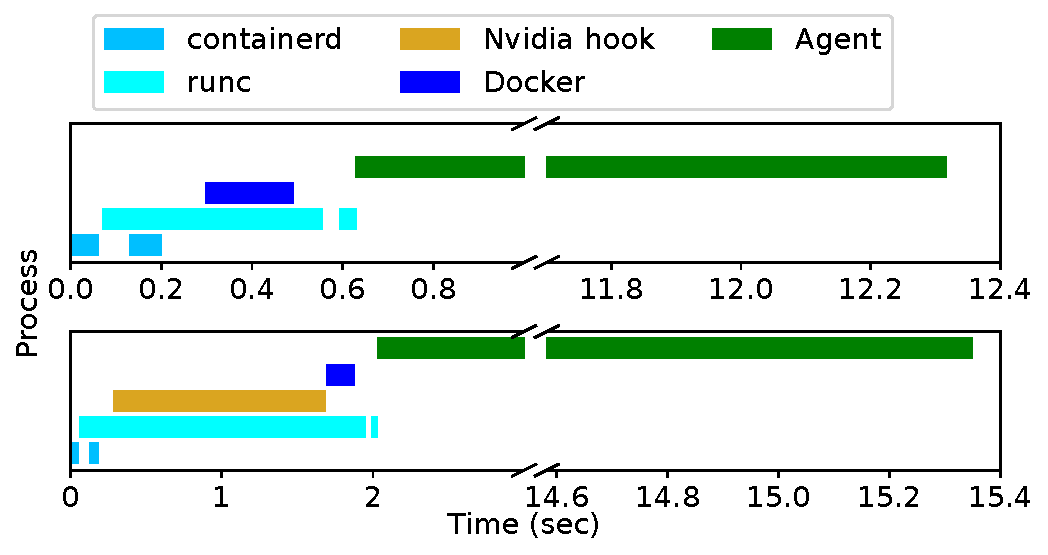
\includegraphics[width=\textwidth]{mqfq/graphs/coldstart/combined_timeline.pdf}
  \caption{Time spent in a cold start without (top) and with (bottom) a GPU attached to a container hosting TensorFlow inference code.
          % Several additional seconds are caused by Nvidia runtimes and user code library loading.
          GPU attachment adds over a second to initialization time, 
          and user code setup of the GPU increases agent startup inside the container. 
          }
    \label{fig:cold-timeline}
% Gunicorn & library load time, no GPU:
% gunicorn: 0:00:11.688722
% Gunicorn & library load time, GPU:
% gunicorn: 0:00:13.320342
% nvidia: 0:00:01.399233
\end{figure}

\subsection{Serverless Scheduling}

% The workloads in FaaS are unique challenge in cloud computing, and make getting good performance out of GPU acceleration a complex challenge.
The workloads in FaaS are highly heterogeneous and represent a unique orchestration challenge in cloud computing.
Memory usage, execution duration, and the inter-arrival-time between invocations can vary by several orders of magnitude~\cite{shahrad2020serverless}.


Previous GPU-enabling works do not address the potential for worker-level queuing of accelerated Serverless functions.
The first proposal~\cite{naranjo2020accelerated} used Docker and only shows performance improvement against CPU runtimes, neither queuing nor any drawbacks from switching computation are considered. 
Several examples~\cite{pemberton2022kernel,gu2023fast,ng2023paella} do schedule ML inference tasks and GPU resources for high GPU utilization, but do so by breaking apart each function to control kernel launches, thereby preclude whole classes of applications from running.

% Existing platforms avoid queuing, and if at all implemented use a simple policy such as FCFS (first-come-first-serve). 
Most scheduling serverless work targets cluster load balancing via locality~\cite{faaslb-hpdc22,kaffes_hermod_2022,abdi2023palette,package-cristina-19}, and avoid queuing at workers.
% A naïve queuing algorithm such as FCFS (first-come-first-serve) or Round Robin works well with CPU scheduling because it can rely on a large pool of containers.
If necessary they use First-Come-First-Serve (FCFS), which works well scheduling on CPUs because it can rely on a large pool of containers to avoid cold starts and expects little queuing of invocations.
Unfortunately, a FCFS policy neither take into account the need for fairness between functions under queuing, nor optimal use of limited device resources.
Moving data between host and device to change the running application is slow, as seen by~\cite{yu2019automatic, hong2017gpu} and we show below in Section~\ref{sec:shim}.
A new scheduling policy that considers locality of data on device and locality of functions in a smaller container warm pool are needed for viable GPU performance.
% Our memory multiplexing and manipulation
% However, the challenge of GPU locality and warm-pool leads these to high rates of cold starts, container churn, and loss of fairness.

% GPU functions also need data to be local

% Maintaining locality has seen much work~\cite{faaslb-hpdc22,kaffes_hermod_2022,abdi2023palette}, all trying to handle the highly heterogeneous~\cite{shahrad2020serverless} workloads of FaaS.
% Inter-arrival-times for functions can vary by several orders of magnitude, as do runtime characteristics such as execution time and memory usage.
% Inter-arrival-times for functions can vary by several orders of magnitude and are not fixed, complicating predicting when and how many containers will be needed.

% The CPU-GPU architecture differences require analyzing how FaaS keeps latency low, and determining how GPUs can fit in.
% Large host memory footprints are taken advantage of by FaaS to run the many containers needed to maintain high locality unpredictable functions.
% Limited GPU memory diminishes the chance for a local container warm hit, highlighting the need for a sizable container pool.
% Recently run functions will also benefit from architecture features like cache presence, and subsequent runs are less likely to need to pull external data dependencies.
% The large number of CPU cores on servers increases invocation concurrency

% A similar correlation exists with GPUs, they run faster when their data is \quotes{local} (i.e. on-device), as we show in our experiments in Section~\ref{sec:shim}.
% We resolve both problems with one solution: oversubscribe device resources and manipulate it for better locality.

% The limited resources of GPUs need a more advanced scheduler to provide \emph{locality}
% Our queue design can run invocations out-of-order, allowing several dispatches of a function in succession to increase warm hits, lowering latency.

GPU batching has been effective~\cite{ali_batch_2020,yang2022infless,ali2022optimizing} in improving GPU utilization and latency when executing ML tasks.
The inputs of multiple invocations are merged into one \emph{batch} by the control plane, computed together, and split apart to distribute results.
% Scientific applications among others are not amenable to batching, and for those that do, they require changing the FaaS paradigm.
Such white-box solutions eschew isolation by making assumptions about the workload, the fact that inputs can be manipulated and how function code can make use of them.
Scientific applications among others are not amenable to batching as their inputs cannot be merged in an attempt at more efficient computation.
Black-box scheduling that works with all application classes is required for generic adoption of accelerators in cloud serverless platforms.


\subsection{Balancing Workloads}

% Serverless relies on \emph{locality} to achieve low latency, a warm container isn't the only factor in this.
% Enabling new worklaods to run on serverless platforms is not sufficient, the workflow must also be fast and unobtrusive. 
% Users expect good \emph{performance} out of the control plane, else they will host their application another way.
% Serverless relies on \emph{locality} to achieve its low latency target, having both a warm container and data be present on-device for optimal results.
% Finally, platforms must be \emph{fair} and prevent function starvation when sharing compute time.

To demonstrate that our system achieves fairness with high performance and locality, we run a trace from our experiments (Sec.~\ref{sec:queue-knobs}) and compare the CPU vs GPU performance.
This representative workload is run on two systems: one with 48 CPU cores, and the other with two Nvidia P100 GPUs.
The functions are restricted to only use one of the two compute types, and the outcome is in Figure~\ref{fig:cpu-compare}.
% The GPU system, despite having lower compute concurrency, has 50\% lower latency 
The GPU system cannot run as many functions concurrently, requiring queuing, but still achieves 50\% lower latency over its CPU-only counterpart.
% These are performance gains and application opportunities which are currently being left on the table by because of the lack of compute parallelism, and which we are the first to enable.

% GPUs have become pervasive as a way of accelerating computation of all types, and are common in cloud computing offerings.
% Yet outside research proposals, they havenot been integrated into serverless computing platforms.
 
\begin{figure}
  \centering
  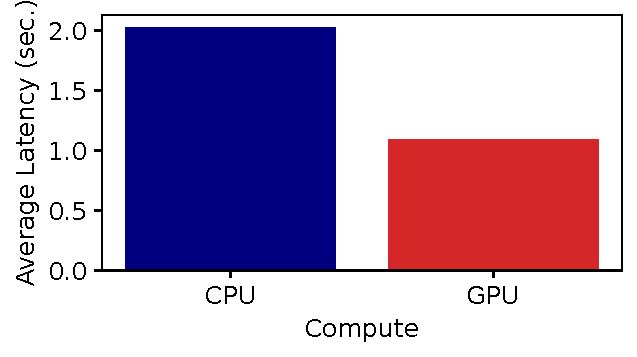
\includegraphics{mqfq/graphs/cpu_compare/25.7/compute_compare_squish.pdf}
  \caption{Average invocation latency for a trace is 2x better on a small GPU platform running our desigin compared to a CPU-only system.}
    \label{fig:cpu-compare}
\end{figure}
